\def\CTeXPreproc{Created by ctex v0.2.9, don't edit!}
%\documentclass{beamer}
\documentclass[%handout,
xcolor=pdftex]{beamer}
\mode<presentation> {
  \usetheme{Warsaw}
  \setbeamercovered{transparent}
}
\let\Tiny=\tiny
\usetheme{Singapore}
\usecolortheme{dolphin}
\usepackage{amsmath}
\usepackage{textcomp}
\usepackage{amssymb}
\usepackage{amsthm}
\usepackage{graphicx}
\usepackage{color}
\usepackage{lipsum}
\usepackage{hyperref}
\usepackage{multirow}
\usepackage{bm}
\DeclareMathSymbol{\Phi}{\mathalpha}{operators}{8}
%\setbeamertemplate{headline}{}
\setbeamertemplate{footline}[page number]
\newcommand\Fontvi{\fontsize{9pt}{8}\selectfont}
\newcommand\Fontvii{\fontsize{7pt}{8}\selectfont}
\newcommand{\backupbegin}{
   \newcounter{finalframe}
   \setcounter{finalframe}{\value{framenumber}}
}
\newcommand{\backupend}{
   \setcounter{framenumber}{\value{finalframe}}
}\newtheorem{proposition}{Proposition}
\title{Unit 17: Introduction to Spectral Analysis}
\author[STAT 5170: Applied Time Series, Unit 17]{Taylor Brown}
\institute{Department of Statistics, University of Virginia}
\date{Fall 2020}

\AtBeginSubsection[] {
  \begin{frame}<beamer>{Outline}
    \tableofcontents[currentsection,currentsubsection]
  \end{frame}
}



\begin{document}


\frame{\titlepage}


\begin{frame}
\frametitle{Readings for Unit 17}

Textbook chapter 4.1.

\end{frame}



% \begin{frame}
% \frametitle{Last Unit}
% \begin{enumerate}
% \item Seasonal Differencing.
% \item Building the Seasonal ARIMA model.
% \end{enumerate}
% \end{frame}

\begin{frame}
\frametitle{Motivation}

There are two primary approaches to time series.  One is the \textbf{time domain} approach, which we covered in Units 8 to 16.  This approach focuses on the rules for a time series to move forward.\\
\vspace{5mm}
The other approach is the \textbf{frequency domain} approach.  This approach tries to understand how differing oscillations can contribute to current observations.

\end{frame}

\section{Introduction to Spectral Analysis}
\frame{\tableofcontents[currentsection]}

\begin{frame}
\frametitle{Time Domain Approach}

Time domain approach: models which give an explicit formula for the current observation in terms of past observations and past white noise terms. ``Regression of the present on the past."

\end{frame}

\begin{frame}
\frametitle{Frequency Domain Approach}

Frequency domain approach: current observation as a combination of waves.  ``Regression of the current  time on sines and cosines of various frequencies."\\
\vspace{5mm}
Idea: decompose a stationary time series $\{x_t\}$ into a \textbf{combination} of sinusoids, with random and uncorrelated coefficients. This is also referred to \textbf{spectral analysis}.


\end{frame}

\begin{frame}
\frametitle{Spectral Analysis}

\begin{itemize}
\item Identify \textbf{dominant frequencies} within the data.
\item Periodogram: \textbf{sample variance} at different of frequencies.
\item Power spectrum: \textbf{population} version of the periodogram.
\end{itemize}


\end{frame}


\begin{frame}
\frametitle{Spectral Analysis}

Period and frequency are inversely related.  
\newline

With quarterly data, there are four data points per year (cycle).  The frequency ($\omega$) 0.25 cycles per data point.  
\newline

The period is
$$
\frac{1}{\omega}
$$

or in this case, $4$.

\end{frame}

\section{Aliasing}
\frame{\tableofcontents[currentsection]}

\begin{frame}
\frametitle{Aliasing}

\begin{itemize}
\item When $\omega=1$, the time series makes one cycle per time unit.
\item When $\omega=0.5$, the time series makes one cycle every two time units.
\item When $\omega=0.25$, the time series makes one cycle every four time units.
\end{itemize}

\end{frame}

\begin{frame}
\frametitle{Aliasing}

Consider cosine curves with $\omega=\frac{1}{4}$ (bold) and $\omega=\frac{3}{4}$ (dashed).

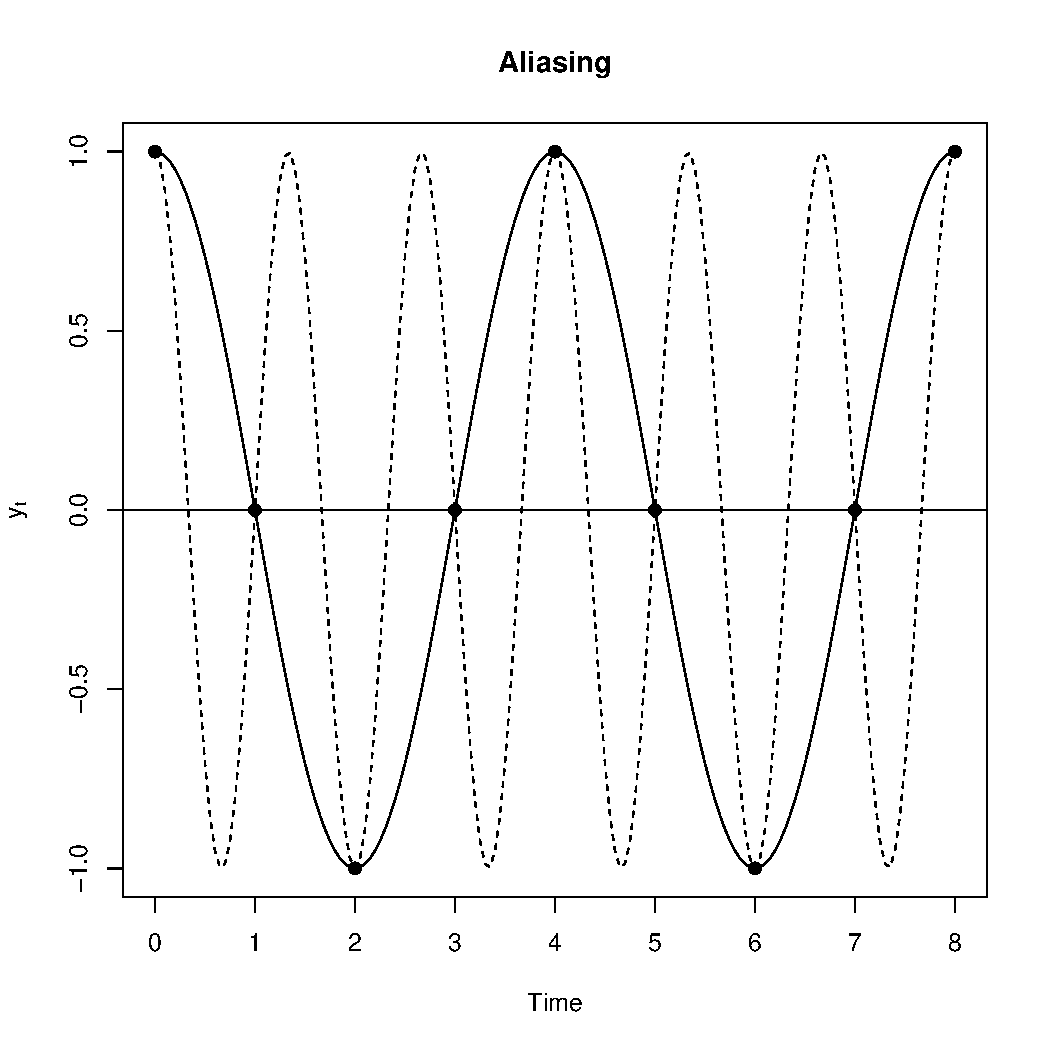
\includegraphics[width=110mm, height=70mm]{alias.pdf}

\end{frame}

\begin{frame}
\frametitle{Aliasing}

Notice that at the discrete time points $0, 1, 2, 3, \cdots$ the two cosine curves have identical values. With \textbf{discrete-time} observations, we would not be able to \textbf{distinguish} between the two curves. So, the frequencies $\frac{1}{4}$ and $\frac{3}{4}$ are \textbf{aliased} with one another.

\end{frame}

\begin{frame}
\frametitle{Aliasing}

This is why we typically focus on frequencies between 0 and 0.5. 
\newline

Higher frequencies may still be present, but they will appear as lower frequencies.


\end{frame}



\section{Periodic Time Series}
\frame{\tableofcontents[currentsection]}

\begin{frame}
\frametitle{Periodic Time Series}

In Unit 6, we discussed periodic functions on the integers that have the following form
$$
x(t)=A \cos(2 \pi \omega t +\phi)
$$
for $t=0, \pm 1, \pm 2, \cdots $ where $\omega$ is the frequency, $A$ is the amplitude, and $\phi$ is the phase.

\end{frame}

\begin{frame}
\frametitle{Some Trigonometric Identities}

\begin{eqnarray*}
\tan(\theta) &=& \frac{\sin(\theta)}{\cos(\theta)}, \\
\sin^2(\theta) + \cos^2(\theta) &=& 1, \\
\sin(a \pm b) &=& \sin(a) \cos(b) \pm \cos(a) \sin(b), \\
\cos(a \pm b) &=& \cos(a) \cos(b) \mp \sin(a) \sin(b).
\end{eqnarray*}

\end{frame}

\begin{frame}
\frametitle{Periodic Time Series}

Having the $\phi$ inside the cosine function can be problematic since if we want to do a regression,
the $\phi$ makes this a non-linear regression. This issue is worked around using a trig identity
$$
\cos(\alpha \mp \beta)=\cos(\alpha) \cos(\beta) \pm \sin(\alpha) \sin(\beta)
$$
to rewrite the periodic function as
\begin{equation} \label{eq:periodic}
x_t=A \cos(\phi) \cos(2 \pi \omega t)-A \sin(\phi) \sin(2 \pi \omega t).
\end{equation}

\end{frame}

\begin{frame}
\frametitle{Periodic Time Series}

Now let's consider (\ref{eq:periodic}) differently from before. Re-write the periodic function (\ref{eq:periodic}) as

\begin{equation} \label{eq:periodic2}
x_t=U_1 \cos(2 \pi \omega t)+U_2 \sin(2 \pi \omega t).
\end{equation}

where $U_1 = A \cos(\phi)$ and $U_2 = -A \sin(\phi)$. We now assume $U_1, U_2$ are iid Gaussian with zero mean and fixed variance.

\end{frame}



\begin{frame}
\frametitle{Periodic Time Series}

Generalize (\ref{eq:periodic2}) to include \textbf{multiple} frequencies and amplitudes with

\begin{equation} \label{eq:gen}
x_t = \sum_{k=1}^{q} U_{k1} \cos(2 \pi \omega_k t) + U_{k2} \sin(2 \pi \omega_k t)
\end{equation}

where the $U_{k1}$ and the $U_{k2}$ are independent and $N(0 , \sigma_k^2)$ and the $\omega_k$ are distinct frequencies.

\end{frame}

\begin{frame}
\frametitle{Periodic Time Series}

A consequence of the representation given by (\ref{eq:gen}) is that any \textbf{stationary} time series may be thought of, approximately, as the random superposition of sines and cosines oscillating at various frequencies.

\end{frame}

\begin{frame}
\frametitle{Periodic Time Series}

Let's derive the moments of (\ref{eq:gen}).

\begin{align*}
E[x_t] &= E[\sum_{k=1}^{q} U_{k1} \cos(2 \pi \omega_k t) + U_{k2} \sin(2 \pi \omega_k t)] \\
&= \sum_{k=1}^{q} E[U_{k1} \cos(2 \pi \omega_k t) + U_{k2} \sin(2 \pi \omega_k t)] \\
&= \sum_{k=1}^{q} E[U_{k1} \cos(2 \pi \omega_k t)] +E[ U_{k2} \sin(2 \pi \omega_k t)] \\
&= \sum_{k=1}^{q} E[U_{k1}] \cos(2 \pi \omega_k t) +E[ U_{k2}] \sin(2 \pi \omega_k t) \\
&= 0
\end{align*}
\vspace{50mm}

\end{frame}

\begin{frame}
\frametitle{Periodic Time Series}


\begin{flalign*}
\gamma(h) &= \text{Cov}\left( x_{t+h}, x_t \right) \\
&= \\
&= \\
&= \\
&= \\
&= \sum_{k=1}^q \sigma^2_k \cos\left(2 \pi \omega_k h \right)
\end{flalign*}


\end{frame}

\begin{frame}
\frametitle{Periodic Time Series}

$$
\gamma(h) = \sum_{k=1}^q \sigma^2_k \cos\left(2 \pi \omega_k h \right)
$$
When we plug in $h=0$, we get
$$
\text{Var}(x_t) = \sum_{k=1}^q \sigma^2_k
$$



\end{frame}

\begin{frame}
\frametitle{Periodic Time Series}

\textbf{Question}: What is the implication of these derivations?
\pause

\begin{equation}
x_t = \sum_{k=1}^{q} U_{k1} \cos(2 \pi \omega_k t) + U_{k2} \sin(2 \pi \omega_k t)
\end{equation}

where $U_{k1}^2 + U_{k2}^2 = A_k^2$. Also $\text{Var}[U_{k1} + U_{k2}] = E[U_{k1}^2] + E[U_{k2}^2] = 2 \sigma_k^2$. 
\pause

Think of it as a regression model:

\begin{equation}
x_t = \sum_{k=1}^{q} \beta_{k1} \cos(2 \pi \omega_k t) + \beta_{k2} \sin(2 \pi \omega_k t)
\end{equation}

$\hat{\beta}_{k1}^2 + \hat{\beta}_{k2}^2$ is the scaled periodogram, it helps estimate $\sigma^2_k$ which is the population parameter corresponding to a realized $A_k^2$.


\end{frame}


\begin{frame}
\frametitle{Next...}

Computing the Fourier transform of the data is faster than fitting a linear regression. 
\newline

Before we discuss that Fourier transform, we'll discuss what happens when you Fourier transform the autocovariance function. This is the ``spectral density."


\end{frame}


\end{document} 